\documentclass{llncs}

\usepackage{llncsdoc}
\usepackage{graphicx,url}
\usepackage[utf8]{inputenc}
\usepackage{float}
\usepackage{setspace}
\usepackage{tabularx}
\usepackage{cite}
\usepackage{hyperref}

\begin{document}
\sloppy
\title{Pushing Together: A platform for social participation}

\author{Tallys Martins\inst{1}, Dylan Guedes\inst{1}, Luan Guimarães\inst{1}\\
        Ricardo Poppi\inst{2}, Henrique Parra\inst{2}, Paulo Meirelles\inst{1}}

\institute{Faculdade do Gama -- Universidade de Brasília (UnB)\\
          Gama/DF -- Brasil\\
  \email{\{tallysmartins,djmgguedes,livreluan\}@gmail.com, paulormm@unb.br}
  \and
          Instituto Cidade Democrática\\
          São Paulo/SP -- Brazil\\
  \email{\{ricardo,henrique\}@cidadedemocratica.org.br}
}
  

\maketitle
\begin{abstract}
  The brazilian government, as many others around the world, has been trying to
build technologies for social collaborative participation, exploring the
guidance of the internet. The participation process is more than just giving
your opinion. It is about dialog and discussion in a way we should have clear
vision on all the sides, all points of view, and all kind of opinions to
discuss what is the best solution to a problem. However, the social networks
and the recommendation systems, in their current design, make a barrier that we
only receive content about what we like, what we follow, and what our friends
like. We are stuck in bubbles of opinion.  With this work we present Pushing
Together, an Open Source platform for collaborative participation that aims for
breaking the bubbles that freezes people in their mindsets. The goal is to
identify different groups of opinion in a conversation using clustering
algorithms, and then give power to some special actors, bringing interaction
between the groups.Through this project, we hope to increase the engagement of
people in terms of social participation and provide new resources for democracy
processes.

\textbf{Keywords:} social participation, open source software, bubbles of
opinion, democracy, gamification
\end{abstract}

\section{Introduction}
\label{sec:intro}
  Promoting social participation is a work made up of many challenges and can
be analyzed from different aspects. Maybe the biggest one is to discover better
ways of keeping the process in domain of both, laypeople and empowered ones,
holding the engagement of the participants.

  Online discussions that happen in standard ways, such as forums/threads, do
not provide an attractive dynamic for those who want to debate. Furthermore, it
is impractical to do any deeper analysis with the generated information, for
example, identify what are the opinion groups formed, or yet which opinion is
majority or minority in discussions that occur in this molds. Making text
analysis, using natural language processing or others techniques, would be an
extremely difficult task given the different themes and contexts of each
conversation, outside the limitations in working with differents idioms.

  In this paper we present the Pushing Together project that applies a
different concept for the debates, called crowdsourced participation, which has
shown to be a great option to break the barriers for engagement and for opening
more space to discussions. With little effort, the participants can give their
opinion from small actions, something comparable to Facebook ``like'' feature.
This way, participation becomes a scalable action for thousands of users in one
click effort.

  Composing people opinion in terms of agree and disagree, 0 or 1, turns
possible the use of clustering algorithms to get sophisticated analysis of what
people think about a subject in a discussion, and this is where Pushing
Together acts.  Analysing formed opinion groups, we identify some profiles seen
as special actors.  Applying concepts of gamification, we give power for those
actors, allowing them to interact in the platform by creating events and
sending direct messages to others. With this strategy, we aim to help to change
the communication and expression of opinion between different groups, facing
what is known as
bubbles\footnote{\url{blog.pol.is/pol-is-in-taiwan-da7570d372b5}} of opinion,
created by nowadays digital media.

\section{Related tool}

  There is a tool called Polis\footnote{\url{pol.is}} that was built on top of
the crowdsourced participation concept and served as inspiration for
development of the Pushing Together project.

  The Polis is a web-based platform that offers to its users the possibility to
reate discussions about any subject. Users can express their point of view in
140 characters comments (Figure \ref{fig:polis-1}). The comments are presented
to users as topics, on cards. The interaction on the system occur by others
participants expressing their agreement or disagreement in existent comments,
or yet by the addition of new ones to the conversation. 

  Representing users opinions as vectors of 0 and 1, Polis applies clustering
algorithms that generates information about the groups of opinion formed, the
most voted proposals, as well as, what proposals were agreed and disagreed by
the most (Figure \ref{fig:polis-2}). 

 \begin{figure}[hbt]
   \centering
   \begin{minipage}{.50\textwidth}
     \includegraphics[width=.9\linewidth]{images/polis1.png}
     \caption{Cards with comments.}
     \label{fig:polis-1}
   \end{minipage}
   \begin{minipage}{.49\textwidth}
     \includegraphics[width=.9\linewidth]{images/polis2.png}
     \caption{Groups of opinion formed.}
     \label{fig:polis-2}
   \end{minipage}
 \end{figure}

  Since Polis did not have the necessary resources for the development of
Pushing Together, we had to implement them, like the identification of the
special profiles inside the clusterization, support to mobile devices, and a
notification system, to name a few. The initial idea was to contribute and
evolve Polis making it possible to achieve the new features. However, their
community was not so open and we had many difficulties through this approach.
The software was miss documented, we had no support from the mainteiners, a
clear sign that they were not interested in our contributions.

  Given the barriers we have found, our tool was born with an independent
architecture, encapsulating Polis in a reverse engineering effort, waiting for
it to evolve or, being more ambitious, aiming to develop our own clustering
service.

\section{The Pushing Together project}
\label{sec:pushingtogether}

  Pushing Together project was born in a kind of a Hackaton. An idea of the
Brazilian non-governmental organization called Cidades Democráticas, which
participated of an event called Collective Intelligence for Democracy, in
Madrid, Spain at the end of 2016.

  With the goal of making the participation an easier process and breaking the
bubbles of opinion, the project makes use of a resource that we named ``the
Push'', which is part of the gamification concept. Users in ownership of this
``power'' will be able to send messages and create events inside the platform.

 \begin{figure}[hbt]
   \centering
     \includegraphics[keepaspectratio=true,scale=0.45]{images/userprofiles.png}
   \caption{User profiles}
   \label{fig:userprofiles}
 \end{figure}

  Making an analysis about the users opinions, we initially identify three
profiles (Figure \ref{fig:userprofiles}) that are considered the potential
receptors for the ``Push'' and some effects that can take place. With this
initial profiles shaping we intend to get a different interaction level between
the multiple opinions in a group of discussion of a participative process.
However, this is still to be tested and validated for consolidation.

 \begin{figure}[hbt]
   \centering
     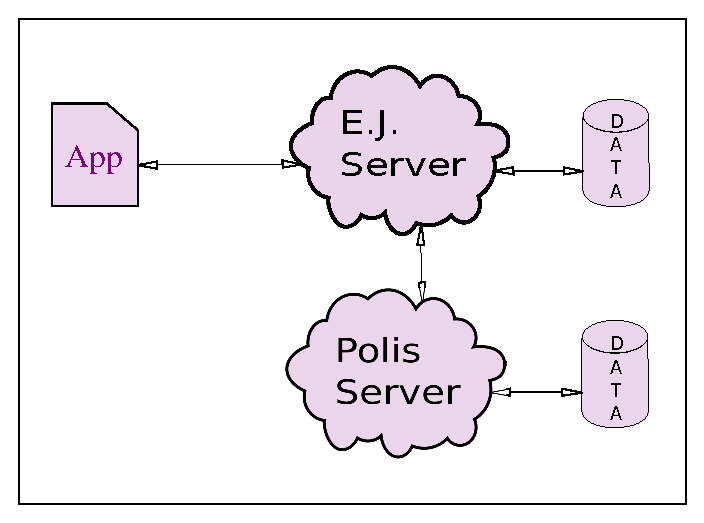
\includegraphics[keepaspectratio=true,,scale=0.5]{images/architecture-1.eps}
   \caption{Architecture of the system}
   \label{fig:architecture-2}
 \end{figure}

  From the technical aspects, the project is divided in a front-end
application, written in React
Native\footnote{\url{facebook.github.io/react-native/}}, and a
NodeJS\footnote{\url{nodejs.org/en/}} server. The server module is responsible
for managing users, the ``Push'' resources in the gamification, and to make the
interface with the external cluster processing service. All the communication,
with the front-end application and the cluster module, is made through an API.
The Figure \ref{fig:architecture-2} below describes this architecture in
general.

\section{Final remarks}

  Pushing Together arise as a potential bridge for dialog between the society
and the state, making different analyzes about the opinion of the distinct
groups and also opening new possibilities for the expression of these opinions
with the ``Push'' resource. Besides, the project was born with transparence and
colaboration principles, building a base for a prospective evolution.

  We are now working on a research for developing a clustering service that will
fit our application model. Parallelly our next steps include finishing the
mobile application using mocked data and validating the user interface.
All this done, a stable version is expected to see the light this year.
  

 %TODO: Próximos passos?

\end{document}
